\documentclass{standalone}
\usepackage{tikz}
\usetikzlibrary{patterns, positioning}

\begin{document}
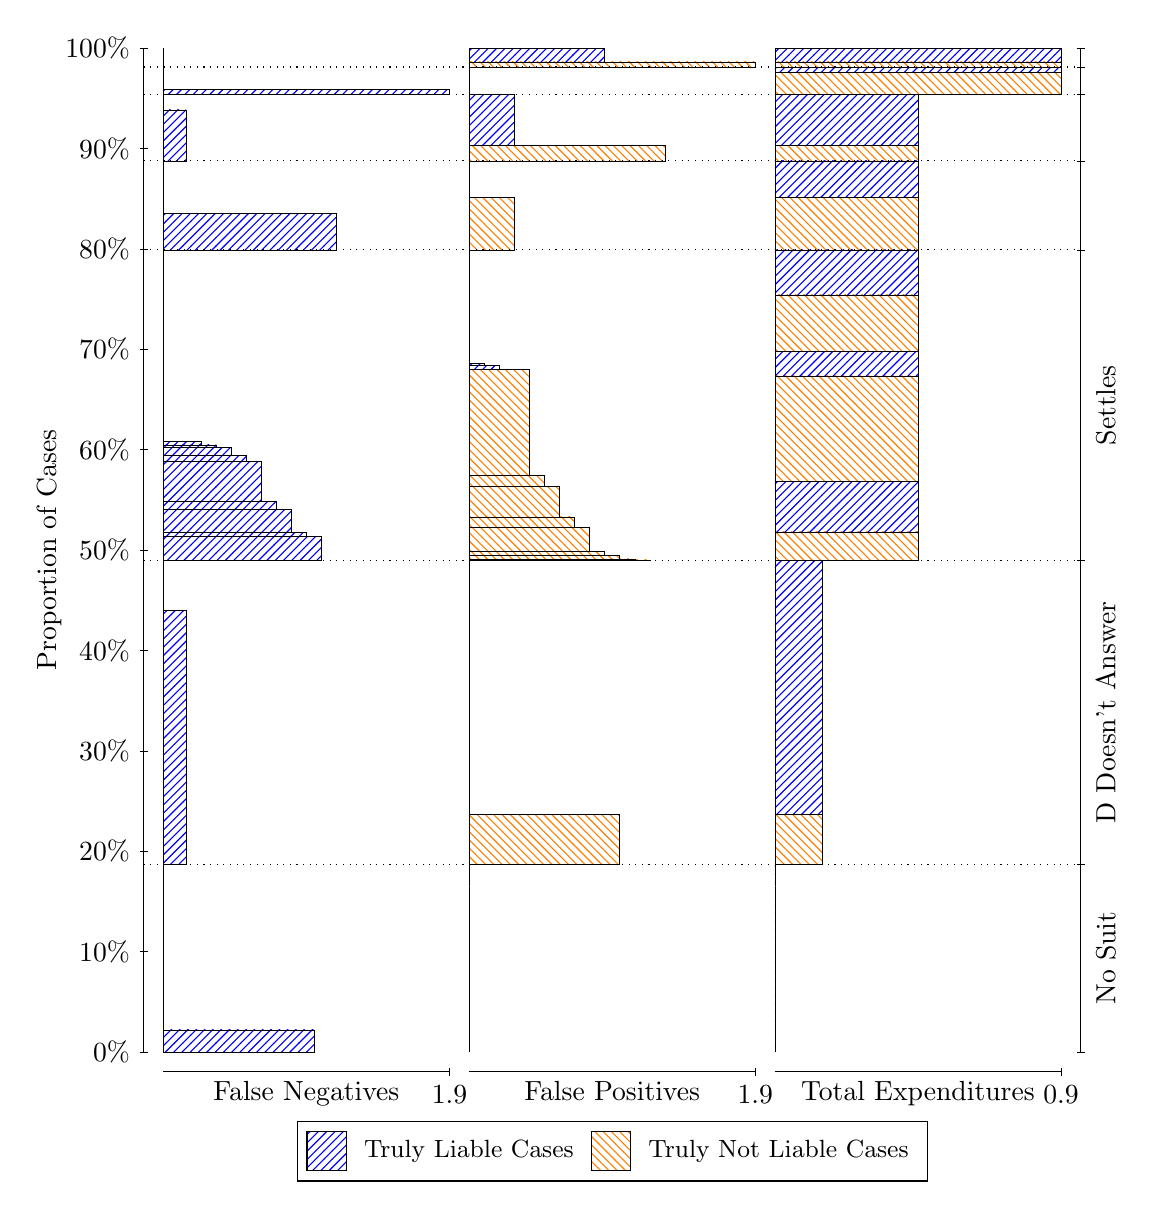
\begin{tikzpicture}
\draw[black, very thin] (1.5,1.75) -- (1.5,14.5);
\node[rotate=90, anchor=center] at (0.3, 8.125) {Proportion of Cases};
\draw[black, very thin] (1.45,1.75) -- (1.55,1.75);
\node[anchor=east] at (1.45, 1.75) {0\%};
\draw[black, very thin] (1.45,3.025) -- (1.55,3.025);
\node[anchor=east] at (1.45, 3.025) {10\%};
\draw[black, very thin] (1.45,4.3) -- (1.55,4.3);
\node[anchor=east] at (1.45, 4.3) {20\%};
\draw[black, very thin] (1.45,5.575) -- (1.55,5.575);
\node[anchor=east] at (1.45, 5.575) {30\%};
\draw[black, very thin] (1.45,6.85) -- (1.55,6.85);
\node[anchor=east] at (1.45, 6.85) {40\%};
\draw[black, very thin] (1.45,8.125) -- (1.55,8.125);
\node[anchor=east] at (1.45, 8.125) {50\%};
\draw[black, very thin] (1.45,9.4) -- (1.55,9.4);
\node[anchor=east] at (1.45, 9.4) {60\%};
\draw[black, very thin] (1.45,10.675) -- (1.55,10.675);
\node[anchor=east] at (1.45, 10.675) {70\%};
\draw[black, very thin] (1.45,11.95) -- (1.55,11.95);
\node[anchor=east] at (1.45, 11.95) {80\%};
\draw[black, very thin] (1.45,13.225) -- (1.55,13.225);
\node[anchor=east] at (1.45, 13.225) {90\%};
\draw[black, very thin] (1.45,14.5) -- (1.55,14.5);
\node[anchor=east] at (1.45, 14.5) {100\%};

\draw[black, very thin] (13.4,1.75) -- (13.4,14.5);
\draw[black, very thin] (13.35,1.75) -- (13.45,1.75);
\node[anchor=west] at (13.35, 1.75) {};
\draw[black, very thin] (13.35,4.1339) -- (13.45,4.1339);
\node[anchor=west] at (13.35, 4.1339) {};
\draw[black, very thin] (13.35,7.9896) -- (13.45,7.9896);
\node[anchor=west] at (13.35, 7.9896) {};
\draw[black, very thin] (13.35,11.936) -- (13.45,11.936);
\node[anchor=west] at (13.35, 11.936) {};
\draw[black, very thin] (13.35,13.067) -- (13.45,13.067);
\node[anchor=west] at (13.35, 13.067) {};
\draw[black, very thin] (13.35,13.909) -- (13.45,13.909);
\node[anchor=west] at (13.35, 13.909) {};
\draw[black, very thin] (13.35,14.259) -- (13.45,14.259);
\node[anchor=west] at (13.35, 14.259) {};
\draw[black, very thin] (13.35,14.5) -- (13.45,14.5);
\node[anchor=west] at (13.35, 14.5) {};

\draw[black, very thin, pattern color=blue, pattern=north east lines] (1.75,1.75) rectangle (3.6623,2.0317);
\draw[black, very thin, pattern color=orange, pattern=north west lines] (1.75,2.0317) rectangle (1.75,4.1339);
\draw[black, very thin, pattern color=blue, pattern=north east lines] (1.75,4.1339) rectangle (2.0368,7.3562);
\draw[black, very thin, pattern color=orange, pattern=north west lines] (1.75,7.3562) rectangle (1.75,7.9896);
\draw[black, very thin, pattern color=blue, pattern=north east lines] (1.75,7.9896) rectangle (3.7579,8.3004);
\draw[black, very thin, pattern color=blue, pattern=north east lines] (1.75,8.3004) rectangle (3.5667,8.3484);
\draw[black, very thin, pattern color=blue, pattern=north east lines] (1.75,8.3484) rectangle (3.3754,8.6408);
\draw[black, very thin, pattern color=blue, pattern=north east lines] (1.75,8.6408) rectangle (3.1842,8.7432);
\draw[black, very thin, pattern color=blue, pattern=north east lines] (1.75,8.7432) rectangle (2.993,9.2496);
\draw[black, very thin, pattern color=blue, pattern=north east lines] (1.75,9.2496) rectangle (2.8018,9.3288);
\draw[black, very thin, pattern color=blue, pattern=north east lines] (1.75,9.3288) rectangle (2.6105,9.4273);
\draw[black, very thin, pattern color=blue, pattern=north east lines] (1.75,9.4273) rectangle (2.4193,9.4586);
\draw[black, very thin, pattern color=blue, pattern=north east lines] (1.75,9.4586) rectangle (2.2281,9.5067);
\draw[black, very thin, pattern color=orange, pattern=north west lines] (1.75,9.5067) rectangle (1.75,11.936);
\draw[black, very thin, pattern color=blue, pattern=north east lines] (1.75,11.936) rectangle (3.9491,12.402);
\draw[black, very thin, pattern color=orange, pattern=north west lines] (1.75,12.402) rectangle (1.75,13.067);
\draw[black, very thin, pattern color=blue, pattern=north east lines] (1.75,13.067) rectangle (2.0368,13.714);
\draw[black, very thin, pattern color=orange, pattern=north west lines] (1.75,13.714) rectangle (1.75,13.909);
\draw[black, very thin, pattern color=blue, pattern=north east lines] (1.75,13.909) rectangle (5.3833,13.975);
\draw[black, very thin, pattern color=orange, pattern=north west lines] (1.75,13.975) rectangle (1.75,14.259);
\draw[black, very thin, pattern color=orange, pattern=north west lines] (1.75,14.259) rectangle (1.75,14.324);
\draw[black, very thin, pattern color=blue, pattern=north east lines] (1.75,14.324) rectangle (1.75,14.5);
\draw[black, very thin, pattern color=orange, pattern=north west lines] (5.6333,1.75) rectangle (5.6333,3.8522);
\draw[black, very thin, pattern color=blue, pattern=north east lines] (5.6333,3.8522) rectangle (5.6333,4.1339);
\draw[black, very thin, pattern color=orange, pattern=north west lines] (5.6333,4.1339) rectangle (7.5456,4.7673);
\draw[black, very thin, pattern color=blue, pattern=north east lines] (5.6333,4.7673) rectangle (5.6333,7.9896);
\draw[black, very thin, pattern color=orange, pattern=north west lines] (5.6333,7.9896) rectangle (7.9281,8);
\draw[black, very thin, pattern color=orange, pattern=north west lines] (5.6333,8) rectangle (7.7368,8.0123);
\draw[black, very thin, pattern color=orange, pattern=north west lines] (5.6333,8.0123) rectangle (7.5456,8.0592);
\draw[black, very thin, pattern color=orange, pattern=north west lines] (5.6333,8.0592) rectangle (7.3544,8.1063);
\draw[black, very thin, pattern color=orange, pattern=north west lines] (5.6333,8.1063) rectangle (7.1632,8.4135);
\draw[black, very thin, pattern color=orange, pattern=north west lines] (5.6333,8.4135) rectangle (6.9719,8.5449);
\draw[black, very thin, pattern color=orange, pattern=north west lines] (5.6333,8.5449) rectangle (6.7807,8.9369);
\draw[black, very thin, pattern color=orange, pattern=north west lines] (5.6333,8.9369) rectangle (6.5895,9.0756);
\draw[black, very thin, pattern color=orange, pattern=north west lines] (5.6333,9.0756) rectangle (6.3982,10.419);
\draw[black, very thin, pattern color=blue, pattern=north east lines] (5.6333,10.419) rectangle (6.0158,10.467);
\draw[black, very thin, pattern color=blue, pattern=north east lines] (5.6333,10.467) rectangle (5.8246,10.498);
\draw[black, very thin, pattern color=blue, pattern=north east lines] (5.6333,10.498) rectangle (5.6333,11.936);
\draw[black, very thin, pattern color=orange, pattern=north west lines] (5.6333,11.936) rectangle (6.207,12.602);
\draw[black, very thin, pattern color=blue, pattern=north east lines] (5.6333,12.602) rectangle (5.6333,13.067);
\draw[black, very thin, pattern color=orange, pattern=north west lines] (5.6333,13.067) rectangle (8.1193,13.262);
\draw[black, very thin, pattern color=blue, pattern=north east lines] (5.6333,13.262) rectangle (6.207,13.909);
\draw[black, very thin, pattern color=orange, pattern=north west lines] (5.6333,13.909) rectangle (5.6333,14.193);
\draw[black, very thin, pattern color=blue, pattern=north east lines] (5.6333,14.193) rectangle (5.6333,14.259);
\draw[black, very thin, pattern color=orange, pattern=north west lines] (5.6333,14.259) rectangle (9.2667,14.324);
\draw[black, very thin, pattern color=blue, pattern=north east lines] (5.6333,14.324) rectangle (7.3544,14.5);
\draw[black, very thin, pattern color=orange, pattern=north west lines] (9.5167,1.75) rectangle (9.5167,3.8522);
\draw[black, very thin, pattern color=blue, pattern=north east lines] (9.5167,3.8522) rectangle (9.5167,4.1339);
\draw[black, very thin, pattern color=orange, pattern=north west lines] (9.5167,4.1339) rectangle (10.122,4.7673);
\draw[black, very thin, pattern color=blue, pattern=north east lines] (9.5167,4.7673) rectangle (10.122,7.9896);
\draw[black, very thin, pattern color=orange, pattern=north west lines] (9.5167,7.9896) rectangle (11.333,8.356);
\draw[black, very thin, pattern color=blue, pattern=north east lines] (9.5167,8.356) rectangle (11.333,8.9923);
\draw[black, very thin, pattern color=orange, pattern=north west lines] (9.5167,8.9923) rectangle (11.333,10.336);
\draw[black, very thin, pattern color=blue, pattern=north east lines] (9.5167,10.336) rectangle (11.333,10.646);
\draw[black, very thin, pattern color=orange, pattern=north west lines] (9.5167,10.646) rectangle (11.333,11.366);
\draw[black, very thin, pattern color=blue, pattern=north east lines] (9.5167,11.366) rectangle (11.333,11.936);
\draw[black, very thin, pattern color=orange, pattern=north west lines] (9.5167,11.936) rectangle (11.333,12.602);
\draw[black, very thin, pattern color=blue, pattern=north east lines] (9.5167,12.602) rectangle (11.333,13.067);
\draw[black, very thin, pattern color=orange, pattern=north west lines] (9.5167,13.067) rectangle (11.333,13.262);
\draw[black, very thin, pattern color=blue, pattern=north east lines] (9.5167,13.262) rectangle (11.333,13.909);
\draw[black, very thin, pattern color=orange, pattern=north west lines] (9.5167,13.909) rectangle (13.15,14.193);
\draw[black, very thin, pattern color=blue, pattern=north east lines] (9.5167,14.193) rectangle (13.15,14.259);
\draw[black, very thin, pattern color=orange, pattern=north west lines] (9.5167,14.259) rectangle (13.15,14.324);
\draw[black, very thin, pattern color=blue, pattern=north east lines] (9.5167,14.324) rectangle (13.15,14.5);
\draw[black, dotted] (1.5,4.1339) -- (13.4,4.1339);
\draw[black, dotted] (1.5,7.9896) -- (13.4,7.9896);
\draw[black, dotted] (1.5,11.936) -- (13.4,11.936);
\draw[black, dotted] (1.5,13.067) -- (13.4,13.067);
\draw[black, dotted] (1.5,13.909) -- (13.4,13.909);
\draw[black, dotted] (1.5,14.259) -- (13.4,14.259);
\draw[black, very thin] (1.75,1.5) -- (5.3833,1.5);
\node[anchor=north] at (3.5667, 1.5) {False Negatives};
\draw[black, very thin] (5.3833,1.45) -- (5.3833,1.55);
\node[anchor=north] at (5.3833, 1.45) {1.9};

\draw[black, very thin] (5.6333,1.5) -- (9.2667,1.5);
\node[anchor=north] at (7.45, 1.5) {False Positives};
\draw[black, very thin] (9.2667,1.45) -- (9.2667,1.55);
\node[anchor=north] at (9.2667, 1.45) {1.9};

\draw[black, very thin] (9.5167,1.5) -- (13.15,1.5);
\node[anchor=north] at (11.333, 1.5) {Total Expenditures};
\draw[black, very thin] (13.15,1.45) -- (13.15,1.55);
\node[anchor=north] at (13.15, 1.45) {0.9};

\node[black, centered, rotate=90] at (13.72, 2.9419) {No Suit};
\node[black, centered, rotate=90] at (13.72, 6.0617) {D Doesn't Answer};
\node[black, centered, rotate=90] at (13.72, 9.9628) {Settles};





\draw (7.449999999999999,1.5) node[draw=none] (baseCoordinate) {};
\begin{scope}[align=center]
        \matrix[scale=0.5, draw=black, below=0.5cm of baseCoordinate, nodes={draw}, column sep=0.1cm]{
            \node[rectangle, draw, minimum width=0.5cm, minimum height=0.5cm, pattern=north east lines, pattern color=blue] {}; &
            \node[draw=none, font=\small] (B) {Truly Liable Cases}; &
            \node[rectangle, draw, minimum width=0.5cm, minimum height=0.5cm, pattern=north west lines, pattern color=orange] {}; &
            \node[draw=none, font=\small] (B) {Truly Not Liable Cases}; \\
            };
\end{scope}

\end{tikzpicture}
\end{document}